\section{Tolérances aux pannes}

\subsection{Présentation générale}

De manière globale, en plus des différents outils utilisés pour la résilience telle que Zookeeper ou HAproxy, cette stack dispose d'un serveur global pour la gestion des pannes. Ce serveur va avoir pour rôle de lancer de manière périodique des vérifications de statuts des différents services deployés. Selon les résultats obtenus, le service pourra être redémarré ou même installé sur une nouvelle machine. De plus pour permettre un suivi facile des erreurs de fonctionnement des statuts, un mail est envoyé dès lors qu'une erreur est détectée. Dans le message du mail est indiqué si l'erreur a pu être résolue de manière automatique.

\subsection{Infrastructure mise en place}
\ \\
\centerline{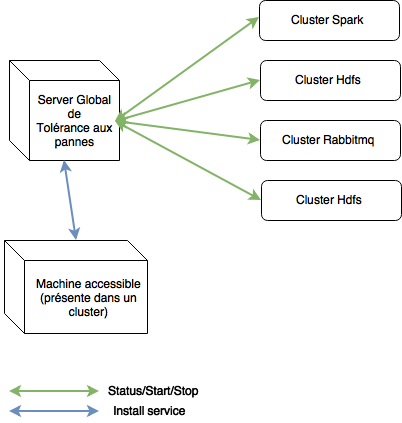
\includegraphics[scale=0.50]{pics/resilience-infra.png}}
\centerline{\caption{Schéma globale de l'infrastructure mise en place pour SPARK}}
\ \\